%Investigar como objetivos de la seguridad de la información o telecomunicaciones
%Intro: Confidencialidad, autenticidad e integridad de las comunicaciones
\section{Seguridad de las comunicaciones}
\label{sec:segDeLasComun}
La seguridad de la información en telecomunicaciones es crucial para proteger los datos en tránsito. En este campo, la confidencialidad, la autenticidad y la integridad de los datos son fundamentales.

La confidencialidad implica la protección de la información sensible contra accesos no autorizados. A través de métodos como la encriptación, se busca garantizar que solo los destinatarios autorizados puedan interpretar la información transmitida, preservando así la confidencialidad de los datos \cite{stallings2016network}

La autenticidad se refiere a la verificación de la identidad de las entidades involucradas en una comunicación. Para este fin, se emplean mecanismos como la autenticación de dos factores y la firma digital, aplicados en distintos contextos. Estos métodos permiten confirmar que emisor y receptor son entidades legítimas, reduciendo el riesgo de suplantación de identidad y garantizando la autenticidad del origen de los mensajes \cite{stallings2016network}. La firma digital es una técnica criptográfica basada en criptografía asimétrica que permite verificar la integridad y autenticidad de un documento electrónico, así como garantizar el no repudio. Asegura que el contenido del documento no ha sido alterado desde su firma y que el firmante no puede negar su autoría. Este mecanismo utiliza un par de claves: una clave privada, conocida únicamente por el firmante, y una clave pública, accesible a terceros para verificar la firma.

La integridad tiene como objetivo garantizar que la información no ha sido alterada ni se ha insertado contenido no autorizado, ya sea por errores accidentales durante la transmisión o por ataques maliciosos. Para ello, se emplean técnicas como los códigos de detección y corrección de errores para fallos involuntarios, y mecanismos criptográficos como funciones hash y códigos de autenticación de mensajes (MAC) para detectar modificaciones intencionadas \cite{stallings2016network, delfsintroduction}.

Éste enfoque integral en confidencialidad, autenticidad e integridad es esencial para proteger la información en las telecomunicaciones y también contribuye a fortalecer la confianza en los sistemas y servicios digitales \cite{stallings2005cryptography,stallings2016network}.

Un campo esencial para la seguridad de la información es la criptografía, donde un mensaje en su forma original se conoce como texto claro mientras que un mensaje transformado y codificado se denomina texto cifrado. La criptografía se fundamenta en principios clave para transformar el texto claro en texto cifrado. Estos principios, presentes en todos los algoritmos de cifrado, se basan en dos operaciones generales: la sustitución, donde cada elemento en el texto claro (bit, carácter, grupo de bits) es reemplazado por otro elemento, y la transposición, donde los elementos en el texto claro se reorganizan. Es crucial que no se pierda información, es decir, que todas las operaciones sean reversibles. La mayoría de los sistemas, conocidos como sistemas de producto, emplean múltiples etapas de sustituciones y transposiciones, formando un producto de operaciones criptográficas.

El proceso de convertir el texto claro en texto cifrado se conoce como cifrado o encriptación, y el acto de restaurar el texto claro a partir del texto cifrado se denomina descifrado o desencriptación.

La forma en que se procesa el texto claro también es un factor determinante porque determina cómo se cifra y descifra la información. Un cifrado de bloque procesa los elementos de entrada en bloques, generando un bloque de salida para cada bloque de entrada. Por otro lado, un cifrado de flujo procesa continuamente los elementos de entrada, produciendo la salida elemento a elemento a medida que avanza \cite{schneier2007applied, stallings2005cryptography}.

La criptografía se clasifica según el número de claves utilizadas. La criptografía simétrica, también conocida como criptografía de clave secreta o criptografía convencional, es fundamental en la seguridad de la información. En éste enfoque, se utiliza una única clave compartida entre las partes autorizadas para cifrar y descifrar datos. La premisa básica radica en mantener esta clave en secreto, asegurando que solo aquellos que poseen dicha clave secreta puedan acceder a la información protegida. 

A partir de la Figura \ref{fig:procesoCifrado} se plantea cómo es el proceso de encriptación y desencriptación de clave simétrica. En esta, se considera que $K_i$ y $K_j$ son la misma clave secreta compartida entre el emisor y el receptor. Esta clave es utilizada por los algoritmos de encriptación y desencriptación para cifrar y descifrar el texto. Los algoritmos de encriptación y desencriptación se encargan de realizar una serie de transformaciones y sustituciones sobre el texto haciendo uso de la clave provista. Este método requiere que la distribución de la clave secreta entre las entidades participantes de la comunicación se realice a través de un canal seguro. La necesidad de un canal seguro es una desventaja del método de clave simétrica, pero a cambio, se tiene el beneficio de ser muy eficiente respecto de los recursos computacionales necesarios para los procesos de cifrado y descifrado.


\begin{figure}
    \centering
    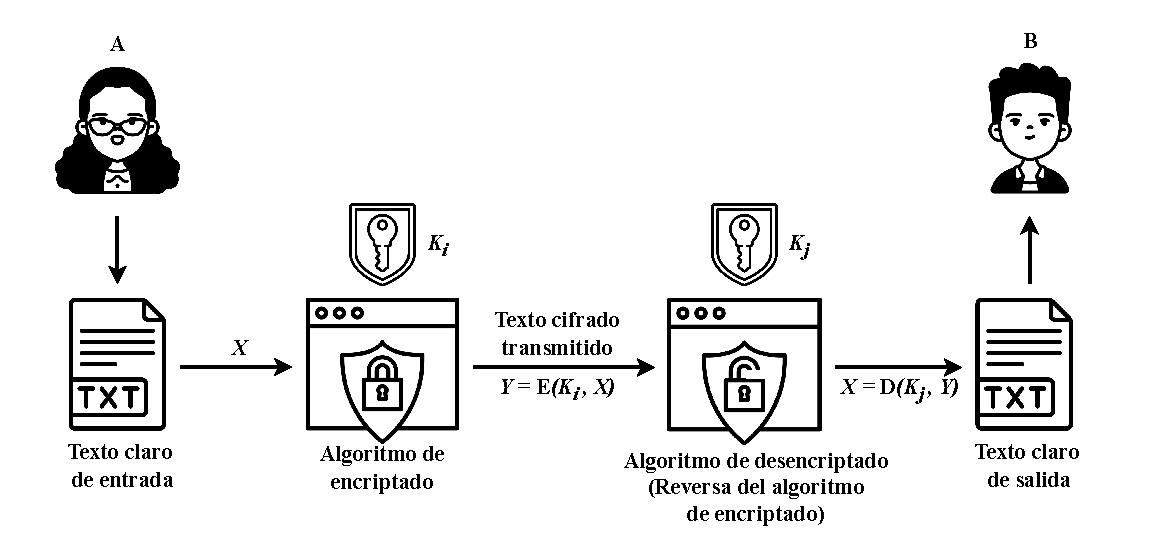
\includegraphics[width=1\linewidth]{Imagenes/Seguridad de las comunicaciones/Cifrado simetrico y asimetrico.pdf}
    \caption{Proceso de encriptación con claves}
    \label{fig:procesoCifrado}
\end{figure}

\subsection{Cifrado asimétrico}
A diferencia del cifrado simétrico, que depende de una clave secreta compartida, la criptografía de clave pública utiliza un par de claves: una \textit{clave pública} y una \textit{clave privada}. La clave pública, como su nombre lo indica, se comparte abiertamente, permitiendo que cualquiera pueda cifrar o descifrar mensajes con ella. Por otro lado, la clave privada, es secreta y solo conocida por el propietario que la generó. En este esquema, lo que se cifra con una de las claves sólo puede ser descifrado con la otra, es decir, no es posible cifrar y descifrar con la misma clave. Esto permite asegurar la confidencialidad de los mensajes, ya que un mensaje cifrado con la clave pública de un usuario sólo puede ser leído por quien posee la clave privada correspondiente.

El funcionamiento esencial para garantizar la confidencialidad se puede ver representado en la Figura \ref{fig:procesoCifrado}, donde $K_i$ es la clave pública de ``B'' y $K_j$ es la clave privada de ``B'' y se describe de la siguiente manera:
\begin{enumerate}
    \item Los usuarios generan pares de claves pública y privada. 
    
    \item Los usuarios obtienen la clave pública del otro con el que se quieren comunicar.

    \item Si ``A'' quiere enviar un mensaje confidencial a ``B'', ``A'' encripta el mensaje utilizando la clave pública de ``B''.

    \item Cuando ``B'' recibe el mensaje, éste lo desencripta utilizando su clave privada. Ninguna otra persona puede desencriptar el mensaje porque solamente ``A'' conoce su clave privada. 
\end{enumerate}

De esta manera, como cualquiera tiene acceso a las claves públicas, se elimina la necesidad de claves secretas compartidas. Siempre que la clave privada de un usuario se mantenga en secreto, la comunicación estará segura. Por otro lado, en caso de necesidad ya sea porque se filtró una clave privada u otra razón, un sistema o usuario puede generar un nuevo par de claves.

Por otro lado existe la necesidad de que los mensajes y documentos electrónicos cuenten con un equivalente a las firmas utilizadas en documentos en papel. Esto se logra con firmas digitales. 

La firma digital de un documento se realiza, de manera conceptual, de la siguiente manera:

\begin{enumerate}
    \item Si ``A'' quiere firmar un mensaje, primero genera un resumen criptográfico del mensaje (mediante una función hash). Luego, cifra ese resumen utilizando su clave privada. El resultado se adjunta al mensaje como su firma digital.

    \item Cuando ``B'' recibe el mensaje junto con la firma, genera él mismo el resumen criptográfico a partir del mensaje recibido. Luego, utiliza la clave pública de ``A'' para descifrar la firma y así obtener el resumen original. Si ambos resúmenes coinciden, se confirma que el mensaje no ha sido alterado y que fue firmado por ``A''.
\end{enumerate}

Cabe destacar que en este ejemplo el mensaje no se cifra, por lo que la firma digital no garantiza la confidencialidad, sino la autenticidad, la integridad y el no repudio del mensaje.

Este esquema garantiza tanto la autenticidad del origen, ya que solo ``A'' posee la clave privada, como la integridad del mensaje, dado que cualquier alteración modificaría el resumen y anularía la verificación de la firma.

La firma digital de un documento se realiza, de manera conceptual, de la siguiente manera:

\begin{enumerate}
    \item Si ``A'' quiere firmar un mensaje, ``A'' encripta el mensaje utilizando su clave privada.

    \item Cuando ``B'' recibe el mensaje, éste lo desencripta utilizando la clave pública de ``A''. Dado que el mensaje fue encriptado con la clave privada de ``A'', solo ``A'' pudo haberlo generado. 
\end{enumerate}

Este esquema planteado asegura que el mensaje no sea alterado sin acceso a la clave privada de A, garantizando así tanto la autenticidad del origen como la integridad del contenido del mensaje.

\subsection{Certificados de claves públicas y verificación de validez de certificados}

%Los certificados de claves públicas permiten asociar una identidad con una clave pública, proporcionando un medio para validar la legitimidad de las entidades y prevenir suplantaciones de identidad durante las transmisiones.

%\label{sec:dirPubCAyCerts}
%Los directorios de claves públicas sirven como repositorios (centralizados o distribuidos) donde los usuarios pueden buscar y obtener claves públicas de otros participantes. Estos facilitan la distribución de claves públicas y respaldan la autenticidad e integridad de las comunicaciones. Al proporcionar un medio para la consulta y verificación de claves públicas, contribuyen a establecer una red de confianza entre los usuarios. 

%Tanto el mantenimiento como la distribución del directorio público es responsabilidad de una entidad u organización externa, a la cual se la denomina autoridad de clave pública o autoridad certificante. 

%El funcionamiento de un directorio público se describe de la siguiente manera:

%\begin{enumerate}
%    \item La autoridad de clave pública mantiene un directorio con un registro que contiene el nombre y la clave pública de cada participante.
%    \item Cada participante registra su clave pública en el directorio público. Este registro debe ser realizado en persona o a través de algún canal de comunicaciones seguro que garantice la autenticidad.
%    \item Los participantes pueden reemplazar claves públicas ya existentes por una nueva cuando lo deseen. Por lo general esto se desea hacer cuando una clave pública fue utilizada para una gran cantidad de datos, evitando así ataques criptoanalíticos, o porque la clave privada asociada se vio comprometida de alguna manera.
%    \item Los participantes acceden de manera electrónica al directorio público. Para hacer esto de manera segura, es necesario que la comunicación entre la autoridad y el participante sea autenticada y segura, y que la clave pública de la autoridad sea obtenida previamente de una fuente confiable, ya sea en persona o a través de un canal de comunicaciones seguro, para garantizar la autenticidad de la autoridad.
%\end{enumerate}

%Para lograr un mayor nivel de seguridad se puede realizar un control más estricto sobre la distribución de las claves. En la Figura \ref{fig:directorioPK} se plantea un escenario donde se asume que una autoridad central mantiene un directorio dinámico de claves públicas de todos los participantes. Además cada participante conoce, y obtiene a través de un canal seguro, la clave pública de la autoridad y dicha autoridad es la única que conoce su propia clave privada. De esta manera se describe el siguiente proceso:

%\begin{figure}
%    \centering
%    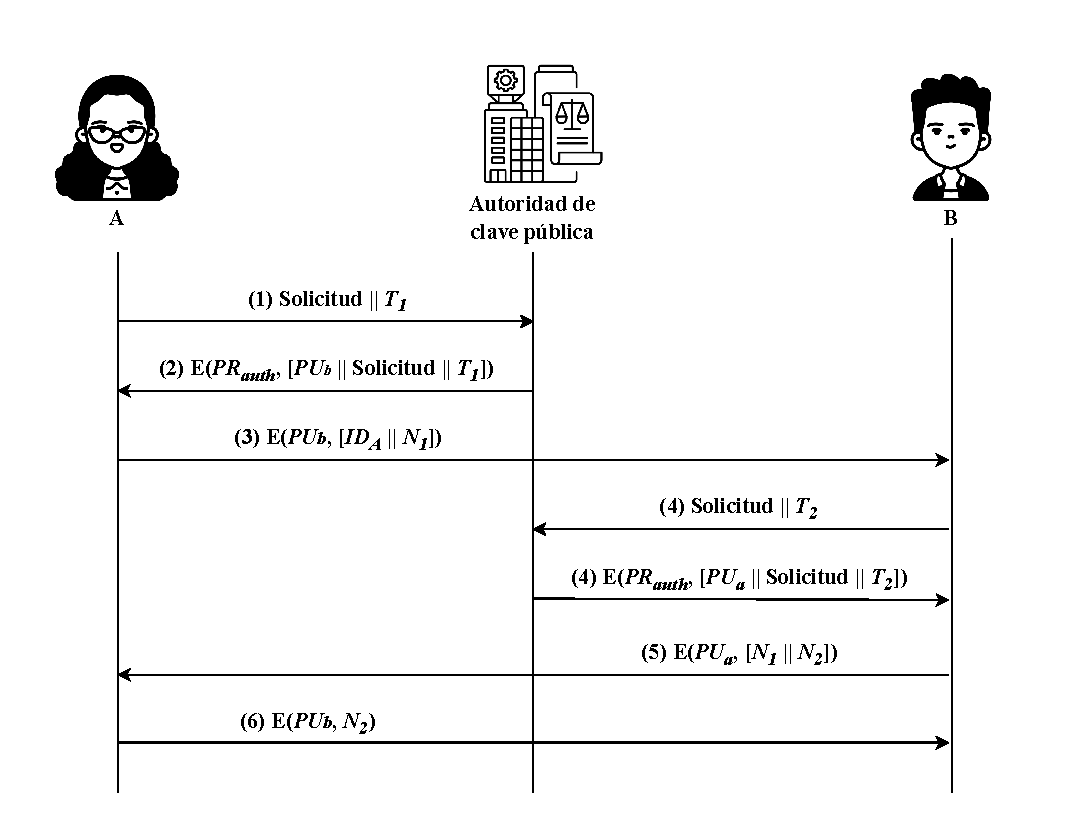
\includegraphics[width=\textwidth]{Imagenes/Seguridad de las comunicaciones/Certificados.pdf}
%    \caption{Escenario de distribución de claves públicas con entidad certificante}
%    \label{fig:directorioPK}
%\end{figure}
%\begin{enumerate}
%    \item ``A'' envía un mensaje de solicitud con marca de tiempo a la autoridad de clave pública pidiendo la clave pública de ``B''.
%    \item La autoridad responde con un mensaje firmado digitalmente con su clave privada. Por lo tanto, ``A'' está segura de que el mensaje fue emitido por la autoridad. El mensaje por parte de la autoridad contiene la siguiente información:
 %   \begin{itemize}
 %       \item Clave pública de ``B'', $PU_b$.
 %       \item La solicitud original. De esta manera ``A'' puede comparar la respuesta con la solicitud original y verificar que no fue adulterada antes de la recepción por parte de la autoridad.
 %       \item La marca de tiempo original. Con esta ``A'' puede determinar si se trata de un mensaje viejo de la autoridad cifrado con otra clave diferente a la clave pública actual de ``B''.
%    \end{itemize}
 %   \item ``A'' almacena la clave pública de ``B'' y la utiliza para encriptar un mensaje con destino a ``B'', agregando su identificador $ID_A$ y un número único ($N_1$), el cual es utilizado para identificar unívocamente la transacción.
 %   \item Utilizando el mismo mecanismo, en caso de ser necesario, ``B'' obtiene la clave pública de ``A''.

%\end{enumerate}
%De esta manera, las claves públicas fueron distribuidas de forma segura tanto a ``A'' como a ``B'', y pueden comenzar un intercambio de información seguro. Finalmente se tienen dos pasos opcionales los cuales verifican que efectivamente ``A'' y ``B'' se están comunicando entre ellos y la clave pública no fue falsificada.
%\begin{enumerate}
%\setcounter{enumi}{4}
%    \item ``B'' envía un mensaje a ``A'', encriptado con la clave pública de esta, es decir $PU_a$, este mensaje contiene el número único de ``A'' ($N_1$) así como un nuevo número único generado por ``B'' ($N_2$). Como solamente ``B'' pudo haber desencriptado el mensaje del paso 3, dado que para ello se requería utilizar su clave privada, la presencia de ($N_1$) en el mensaje de este paso le asegura a ``A'' que el emisor es ``B''.
%    \item ``A'' retorna ($N_2$), el cual es encriptado con la clave pública de ``B'', para asegurarle a ``B'' que el mensaje efectivamente fue emitido por ``A''.
%\end{enumerate}

%De los 6 pasos planteados, los primeros 4 primeros se realizan de forma poco frecuente ya que tanto ``A'' como ``B'' pueden guardar las claves públicas para usos futuros. De todas maneras, es recomendable que los usuarios soliciten periódicamente copias ``frescas'' de claves públicas a sus autoridades correspondientes.



Para garantizar comunicaciones seguras en redes abiertas, es necesario asociar de forma confiable una clave pública con la identidad de su propietario. Esta asociación se logra mediante los \textit{certificados digitales}, que permiten a los usuarios verificar la legitimidad de las claves públicas sin necesidad de consultar constantemente a una autoridad central.

Un certificado digital está compuesto, en esencia, por una clave pública y un identificador del dueño de la clave. Estos elementos conforman un bloque de información que es firmado por un tercero de confianza utilizando su propia clave privada. Típicamente, este tercero es una autoridad certificante (CA), como agencias gubernamentales o instituciones financieras reconocidas por la comunidad.

En la Figura \ref{fig:CADist} se puede ver un ejemplo de emisión de certificados, en esta, los usuarios presentan sus claves públicas a la autoridad a través de un medio seguro con el objetivo de obtener un certificado. La autoridad genera y firma el certificado, representado en la figura con las expresiones del tipo $E(PR_{auth},[T_1||ID_A||PU_a])$, y lo entrega a través del mismo medio. Luego, el usuario puede publicar o compartir este certificado. Cualquier otro que requiera de la clave pública del usuario puede obtener el certificado y verificar que este sea válido mediante la firma adjunta de la entidad certificante haciendo uso de una copia propia de la clave pública de la misma entidad. Además, a los certificados se les asigna una marca de validez temporal. Si una entidad certificante cambia su clave privada, deberán actualizarse todos los certificados firmados con esta.

\begin{figure}
    \centering
    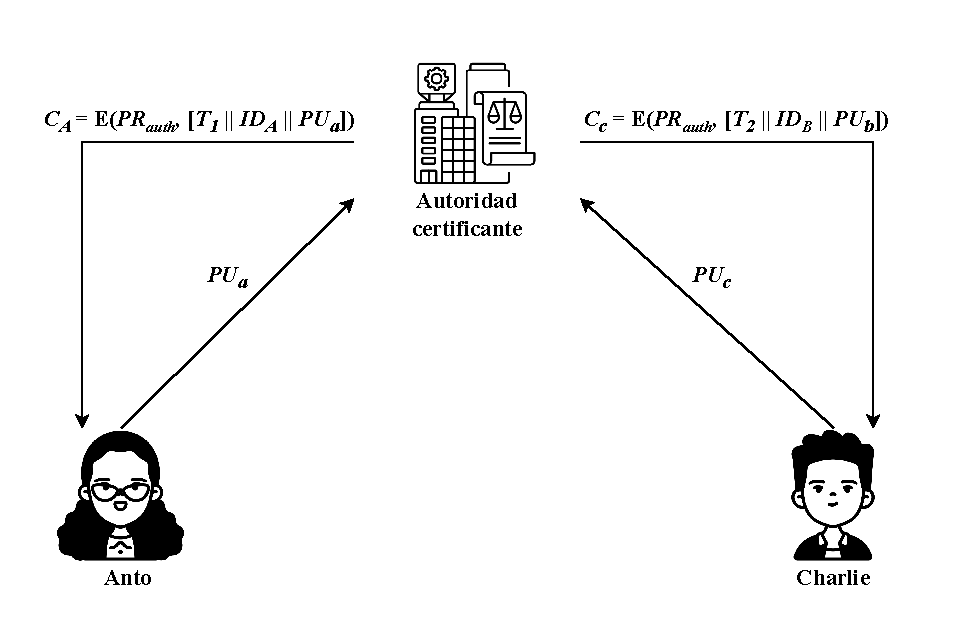
\includegraphics[width=\textwidth]{Imagenes/Seguridad de las comunicaciones/EntidadCertificante.pdf}
    \caption{Distribución de certificados desde la autoridad certificante}
    \label{fig:CADist}
\end{figure}

\textbf{Existen dos tipos principales de autoridades certificantes:}

\begin{itemize}
    \item \textit{Autoridad Certificante Pública:} Es una entidad reconocida globalmente (por ejemplo, por navegadores y sistemas operativos), que emite certificados confiables sin requerir configuración adicional por parte de los usuarios.
    \item \textit{Autoridad Certificante Privada:} Emite certificados dentro de una organización o sistema cerrado. Su uso requiere que los sistemas clientes confíen explícitamente en su clave pública. Se utilizan en entornos corporativos o internos.
\end{itemize}


El uso de certificados digitales da lugar a diferentes configuraciones de infraestructuras de claves públicas como por ejemplo \cite{chokhani2003internet, linn2000trust}:
\begin{itemize}
    \item \textbf{\textit{PKI} Jerárquica:} Hay una autoridad raíz que es la entidad más confiable y, debajo de ella, existen varias entidades subordinadas. Esta configuración permite la delegación de responsabilidades a través de una cadena de confianza establecida a través de certificados.
    \item \textbf{\textit{PKI} en Malla:} Varias entidades certificantes están interconectadas y se reconocen mutuamente, creando una red de confianza, siendo más flexible y descentralizada que las \textit{PKI} jerárquicas ya que no existe una única entidad central.
\end{itemize}

Los certificados autofirmados son generados y firmados por la propia entidad que los utiliza, sin la intervención de una entidad certificante externa. Estos certificados son útiles en entornos propios, donde se requiere cifrado pero no se necesita la verificación por una entidad de confianza externa. En estos entornos, aunque cualquier entidad pueda crear un certificado autofirmado, la autenticidad y seguridad de las comunicaciones se mantienen al confiar en la infraestructura interna de la organización \cite{kumar2019security, cooper2008internet}.


%Por otro lado existen los denominados \textit{certificados autofirmados}, los cuales no son emitidos por una entidad certificante externa, sino que son generados y firmados por la propia entidad que los utilizará. Estos certificados son útiles en situaciones donde se necesita cifrado pero no se requiere la verificación por una entidad de confianza externa. El hecho de que cualquier entidad pueda crear un certificado auto firmado compromete la autenticidad y seguridad de la comunicación, ya que no hay una entidad confiable que valide la autenticidad del certificado. Para mitigar estos riesgos, se pueden implementar infraestructuras de clave pública interna o utilizar mecanismos como el \textit{pinning} para garantizar que solo los certificados específicos y esperados sean aceptados por la aplicación.

\subsubsection{Método de verificación segura mediante pinning de certificados}
La técnica denominada \textit{pinning} permite especificar exactamente en qué entidades se puede confiar, esto a través de la comparación de certificados. Para esto se deben realizar los siguientes pasos:

\begin{enumerate}
    \item \textbf{Almacenamiento del certificado de confianza: }El receptor almacena previamente un certificado de confianza o un hash\footnote{En criptografía, un hash es una función que convierte una entrada arbitraria en una cadena de caracteres de longitud fija.} de ese certificado que recibió a través de un canal seguro.
    \item \textbf{Envío del certificado por el emisor: }Cuando el emisor inicia una conexión, envía su certificado digital al receptor para su validación.
    \item \textbf{Verificación y coincidencia: }El receptor verifica el certificado recibido comparándolo con el certificado de confianza almacenado. Si el certificado enviado por el emisor coincide con el certificado almacenado, se verifica la autenticidad de la conexión. Si no coincide, la conexión se rechaza, previniendo así ataques de hombre en el medio o suplantaciones
\end{enumerate}

Este método asegura que el receptor confía únicamente en un conjunto específico de certificados, lo cual añade una capa extra de seguridad en las comunicaciones. El \textit{pinning} es particularmente útil en aplicaciones sensibles donde la seguridad es crítica y se necesita prevenir ataques que explotan vulnerabilidades en la cadena de confianza de los certificados \cite{stallings2005cryptography, ristic2014bulletproof}.


\subsection{Transport Layer Security (TLS)}
\label{sec:TLS}
TLS es un protocolo criptográfico diseñado para proveer una comunicación segura sobre una infraestructura insegura garantizando:

\begin{enumerate}
    \item \textbf{Confidencialidad: }Mediante el uso de cifrado, TLS intenta garantizar que los datos transmitidos entre el cliente y el servidor no puedan ser interpretados por terceros no autorizados.
    \item \textbf{Integridad: }Mediante el uso de mecanismos criptográficos, como cifrados \textit{AEAD (Authenticated Encryption with Associated Data)}, TLS intenta asegurar que los datos no hayan sido alterados, ni creados, durante la transmisión.
    \item \textbf{Autenticidad: }A través del uso de certificados digitales y la autenticación del servidor, TLS verifica la identidad de las partes que se comunican, asegurando que se está hablando con la entidad correcta.
\end{enumerate}

En la Figura \ref{fig:OSI} se muestra el modelo de Interconexión de Sistemas Abiertos (OSI), un modelo conceptual utilizado para describir cómo se comunican los sistemas en red. Este modelo organiza sus funciones en siete capas jerárquicas, donde cada capa se apoya en los servicios de la inferior. La capa más baja se encarga de la transmisión física de datos, mientras que la capa más alta, la de aplicación, es la que interactúa directamente con el software del usuario y gestiona los datos de las aplicaciones. De esta manera, los protocolos no necesitan preocuparse por la funcionalidad implementada por las capas inferiores. Además, los protocolos en diferentes capas pueden agregarse y eliminarse. Un protocolo en una capa inferior puede ser utilizado por muchos protocolos de niveles superiores. 

\begin{figure}
    \centering
    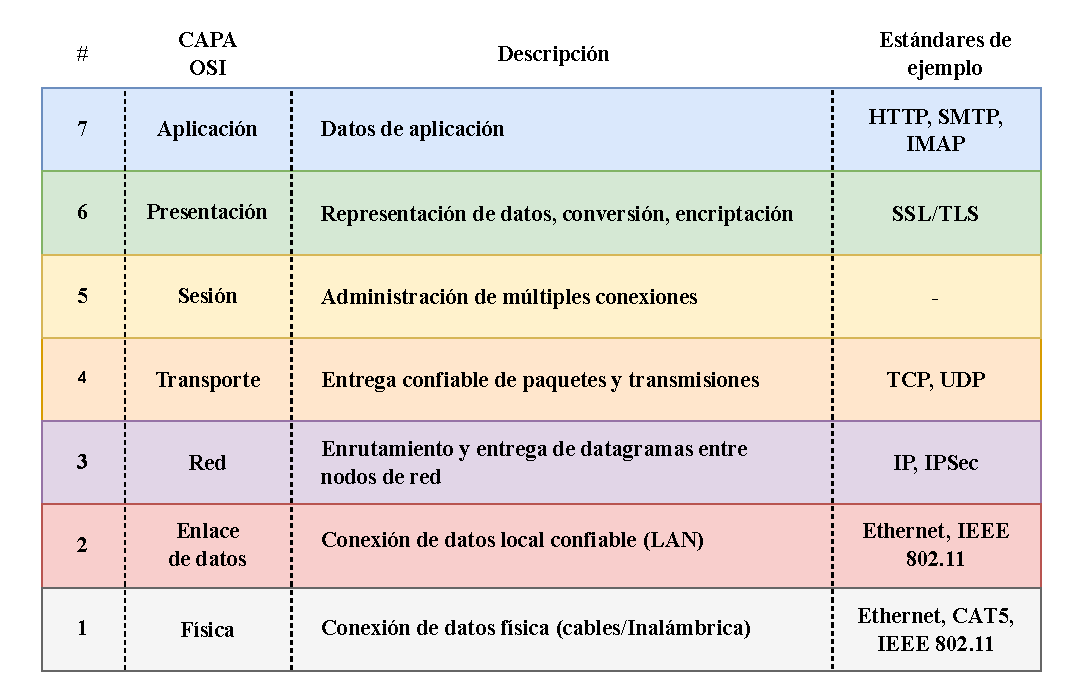
\includegraphics[width=1\linewidth]{Imagenes/Seguridad de las comunicaciones/OSI.pdf}
    \caption{Modelo de Interconexión de Sistemas Abiertos (OSI)}
    \label{fig:OSI}
\end{figure}


Así TLS se sitúa por encima de TCP pero por debajo de protocolos de nivel superior como HTTP pudiéndose utilizar para cifrar HTTP, pero también cualquier otro protocolo que trabaje sobre TCP, como SMTP o IMAP. Cuando no es necesario el cifrado, se puede eliminar TLS del modelo, de manera tal que no afecte a los protocolos de nivel superior, que continuarán funcionando sobre TCP. \cite{ristic2014bulletproof}. 

Aunque hasta aquí se ha utilizado el modelo OSI para describir la arquitectura de red, en la práctica el modelo TCP/IP es el más utilizado. Este modelo, más simplificado y representado en la figura \ref{fig:tcp_ip-tls}, no contempla explícitamente una capa de seguridad. Por esta razón, TLS se suele ubicar entre las capas de aplicación y transporte, actuando como una capa adicional de seguridad superpuesta a la capa de transporte. Esto permite que protocolos como HTTP se ejecuten de forma segura, mejorando así las capacidades del modelo TCP/IP \cite{tracy2002guidelines}.

\begin{figure}
    \centering
    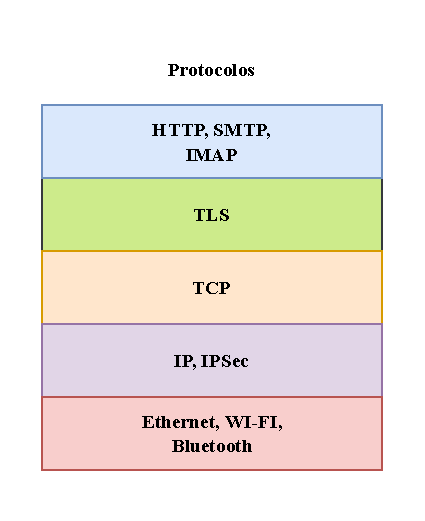
\includegraphics[width=0.5\linewidth]{Imagenes/Seguridad de las comunicaciones/TCP_IP-TLS.pdf}
    \caption{Ubicación de SSL/TLS en la pila de protocolos de Internet}
    \label{fig:tcp_ip-tls}
\end{figure}

Los principios de diseño del protocolo TLS se definen como \cite{ristic2014bulletproof}:
\begin{itemize}
    \item \textbf{Interoperabilidad: }Programadores independientes deben ser capaces de desarrollar programas y librerías que son capaces de comunicarse con otras utilizando parámetros criptográficos comunes, garantizando así la compatibilidad entre versiones TLS. La adopción de estándares abiertos y ampliamente aceptados facilita esta interoperabilidad.
    
    %Esto asegura que las distintas implementaciones de TLS sean compatibles entre sí. La adopción de estándares abiertos y ampliamente aceptados facilita esta interoperabilidad, garantizando que las aplicaciones puedan negociar y abordar protocolos, algoritmos y configuraciones de seguridad compatibles, sin importar su origen o entorno de desarrollo
    \item \textbf{Extensibilidad: }TLS tiene una arquitectura flexible que permite actualizar los algoritmos de cifrado y hash que utiliza, sin necesidad de rediseñar el protocolo completo.

    \item \textbf{Eficiencia: }TLS permite seleccionar algoritmos de cifrado y hash eficientes, lo que ayuda a minimizar el impacto de las operaciones criptográficas en el desempeño del sistema.

\end{itemize}

Toda conexión TLS comienza con un \textit{handshake}. Si el cliente nunca estableció una sesión con el servidor, ambos lados van a ejecutar un \textit{handshake} completo para negociar una \textit{sesión TLS}. Una sesión TLS es el conjunto de parámetros de seguridad acordados entre un cliente y un servidor tras completar un \textit{handshake}. Incluye la versión de TLS utilizada, el conjunto completo de algoritmos de cifrado seleccionado y las claves criptográficas que se usarán durante la comunicación. Una vez establecida, la sesión permite transmitir datos de manera segura mediante cifrado simétrico, garantizando la confidencialidad e integridad de los mensajes. Las sesiones pueden ser efímeras (válidas por una sola conexión) o reanudables, si ambas partes acuerdan reutilizar ciertos parámetros en futuras conexiones para reducir el tiempo de establecimiento.

Durante el \textit{handshake} TLS se realiza un intercambio de claves, cuyo objetivo es establecer una clave simétrica compartida entre cliente y servidor. Para lograrlo, se utiliza criptografía asimétrica o técnicas de intercambio seguro. Estas permiten que ambas partes acuerden una clave sin necesidad de transmitirla directamente. Una vez establecida esta clave simétrica, se emplea el cifrado simétrico para proteger la sesión, ya que este tipo de cifrado es mucho más eficiente computacionalmente para grandes volúmenes de datos. La criptografía asimétrica, se limita a la fase inicial de establecimiento de la sesión, debido a su mayor carga computacional.

Para negociar una nueva \textit{sesión TLS}, el cliente y el servidor realizan las siguientes cuatro actividades:

\begin{enumerate}
    \item Intercambio de capacidades y acuerdo de los parámetros de conexión deseados.
    \item Validación de los certificados presentados o autenticación mediante otros medios.
    \item Acuerdo de un \textit{secreto maestro} compartido entre ambas partes, el cual será utilizado para el cifrado durante la sesión, esta clave es denominada clave de sesión.
    \item Verificar que los mensajes emitidos durante el \textit{handshake} no fueron modificados por un tercero.
\end{enumerate}

En caso de que el cliente ya haya establecido una sesión previa con el servidor, y ambos conservan los datos necesarios, pueden realizar un \textit{handshake} abreviado, reduciendo el tiempo y el consumo de recursos. En la Figura \ref{fig:handshakeTLS} se puede observar el proceso de \textit{handshake} completo donde se describen los mensajes del protocolo.

\begin{figure}
    \centering
    \includegraphics[width= \textwidth]{Imagenes/Seguridad de las comunicaciones/handshakeTLS.pdf}
    \caption{Intercambio de mensajes del \textit{handshake} TLS. Figura extraída de} \cite{ristic2014bulletproof}.
    \label{fig:handshakeTLS}
\end{figure}
\begin{enumerate}
    
    \item \textbf{ClientHello: } Es utilizado para comunicar las capacidades del cliente y sus preferencias al servidor. Siempre es el primer mensaje de cualquier \textit{handshake} TLS. Los clientes envían este mensaje al inicio de nuevas conexiones, cuando intentan renegociar por propia decisión o en respuesta a solicitudes de renegociación por parte del servidor. A partir de este mensaje el servidor elige la versión TLS y el conjunto de cifrado que se va a utilizar en la comunicación. Cabe aclarar que TLS 1.3 eliminó la renegociación, por lo que solo TLS 1.2 y anteriores lo permiten.

    \item \textbf{ServerHello: }El propósito del mensaje \texttt{ServerHello} es comunicar los parámetros de conexión seleccionados por parte del servidor al cliente.



    \item \textbf{Certificate: }El mensaje \texttt{Certificate} se utiliza para enviar una cadena de certificados X.509 \cite{housley1999rfc2459}. Generalmente es enviado por el servidor para permitir su autenticación por parte del cliente. La cadena de certificados incluye, en orden, el certificado del servidor, los intermedios y, opcionalmente, el certificado raíz. Cada certificado en la cadena depende del siguiente para verificar su validez, por lo que la omisión de alguno puede impedir la autenticación.

    Este mensaje es obligatorio cuando el conjunto de algoritmos utilizados requiere autenticación basada en certificados, como ocurre en la mayoría de los casos para autenticar al servidor. Si el cliente no recibe el certificado y no lo tiene almacenado previamente (por ejemplo, mediante una estrategia de pinning), no podrá autenticar al servidor, comprometiendo así una de las propiedades fundamentales de TLS.
    
    Además, el mensaje \texttt{Certificate} también puede ser enviado por el cliente, si el servidor lo solicita, para realizar autenticación mutua mediante certificados.


    \item \textbf{ServerKeyExchange: }El propósito del mensaje \texttt{ServerKeyExchange} es transportar información adicional necesaria para el intercambio de claves. Su contenido varía y depende del conjunto de cifrado negociado.

    \item \textbf{ServerHelloDone: }Es una señal de que el servidor ya envió todos sus mensajes correspondientes al \textit{handshake}. Después de esto, el servidor espera mensajes por parte del cliente.

    \item \textbf{ClientKeyExchange: }Contiene la información relativa al intercambio de claves por parte del cliente. Es obligatorio y su contenido varía y depende del conjunto de cifrado negociado. Una vez recibido por parte del servidor se procede con la generación de las claves de sesión.

    \item \textbf{ChangeCipherSpec: }Es una señal de que el emisor obtuvo la información suficiente para construir los parámetros de conexión, generar las claves de sesión, y proceder con la encriptación. Tanto el cliente como el servidor envían este mensaje.

    \item \textbf{Finished: }Indica que el \textit{handshake} está completo. El cliente envía un código de autenticación de mensajes (MAC) \cite{bellare1996keying, stallings2005cryptography} de todos los mensajes del protocolo de enlace TLS que ha enviado y recibido hasta ese punto. Esto con el objetivo de verificar la integridad y la autenticidad de todos los mensajes intercambiados durante el proceso de \textit{handshake}.
\end{enumerate}

Una vez establecido el \textit{handshake} de TLS, las comunicaciones entre el cliente y el servidor quedan cifradas y seguras.

